\documentclass[12pt]{article}

\usepackage{caption}
\usepackage{subcaption}
\usepackage{float}
\usepackage{makecell}
\usepackage{amsmath}
\usepackage{graphicx}
\graphicspath{ {./images/} }
\usepackage[utf8]{inputenc}
\usepackage[russian]{babel}
\usepackage{geometry}
 \geometry{
 a4paper,
 left=20mm,
 right=20mm,
 top=20mm,
 bot=20mm,
 }

\begin{document}

\begin{titlepage}
\begin{center}
    {\small НАЦИОНАЛЬНЫЙ ИССЛЕДОВАТЕЛЬСКИЙ УНИВЕРСИТЕТ ИТМО} \\
    {\small Факультет систем управления и робототехники} \\
    \vspace*{10\baselineskip}
    {\LARGEЭлектроника и схемотехника} \\
    \ \\
    {\LARGEЛабораторная работа №1} \\
    \ \\
    {\LARGEИсследование полупроводникового диода} \\
    \ \\
    Вариант 2 \\
    \vspace*{10\baselineskip}
    \hfill {\small Выполнили студенты:} \\
    \hfill {\small Кирбаба Д.Д. R3338} \\
    \hfill {\small Курчавый В.В. R3338} \\
    \ \\
    \hfill {\small Преподаватель:} \\
    \hfill {\small Николаев Н.А.} \\
    \mbox{}
    \vfill {\smallг. Санкт-Петербург\\2023}
\end{center}
\end{titlepage}

\section*{Цель работы}
\begin{itemize}
  \item Исследование вольтамперной характеристики (ВАХ) полупроводникового диода;
  \item Исследование работы однополупериодного выпрямителя;
  \item Исследование работы мостового выпрямителя.
\end{itemize}

\section*{Ход работы}
Вариант 2: диод ES1D.
\begin{figure}[H]
    \centering
    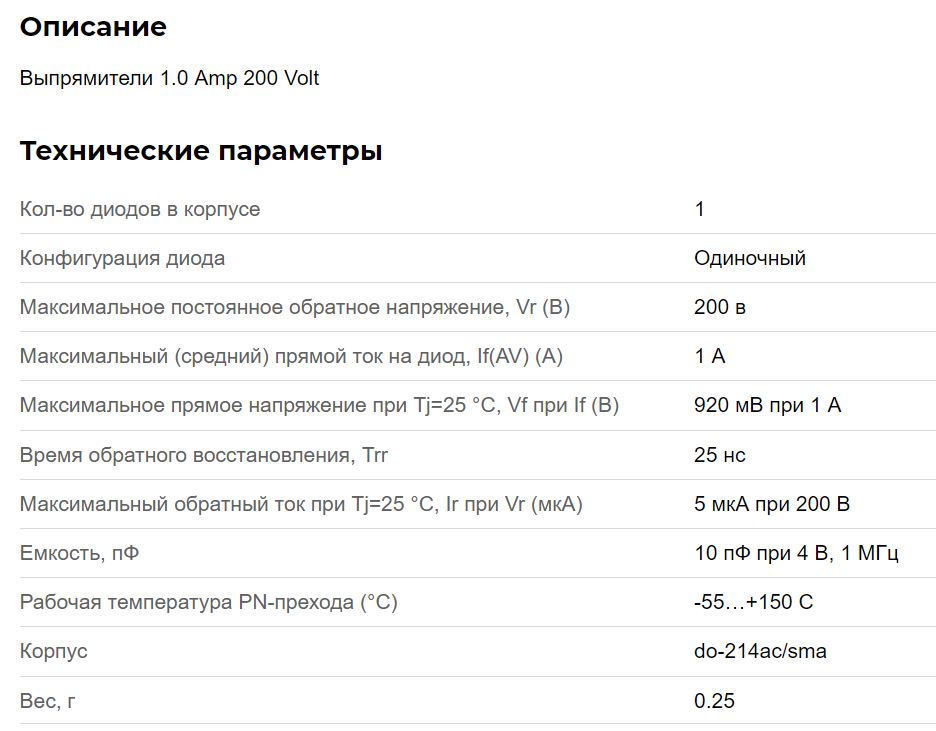
\includegraphics[width=0.7\textwidth]{es1d_params.png}
    \caption{Характеристики диода.}
    \label{fig:es1d_params.png}
\end{figure}\\

\subsubsection*{Исследование ВАХ полупроводникового диода}
Построим прямую ветвь ВАХ полупроводникового диода ES1D (шаг напряжения $0.001 A$).
\begin{figure}[H]
    \centering
    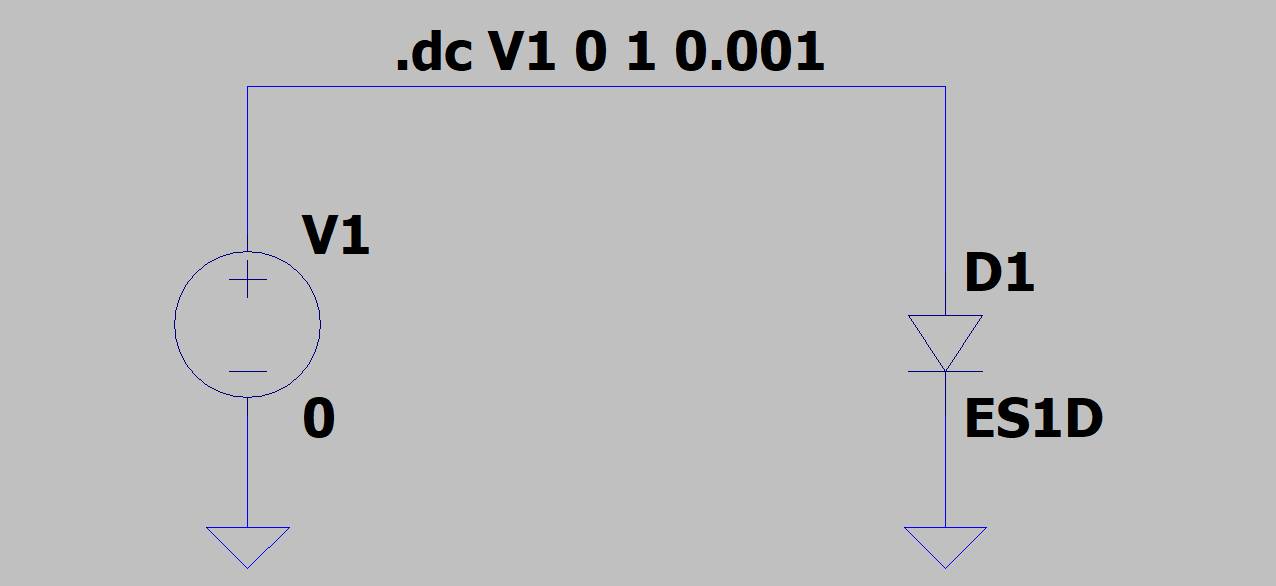
\includegraphics[width=0.7\textwidth]{1_1_circuit_scheme.png}
    \caption{Принципиальная схема для моделирования ВАХ диода.}
    \label{fig:1_1_circuit_scheme.png}
\end{figure}\\

\begin{figure}[H]
    \centering
    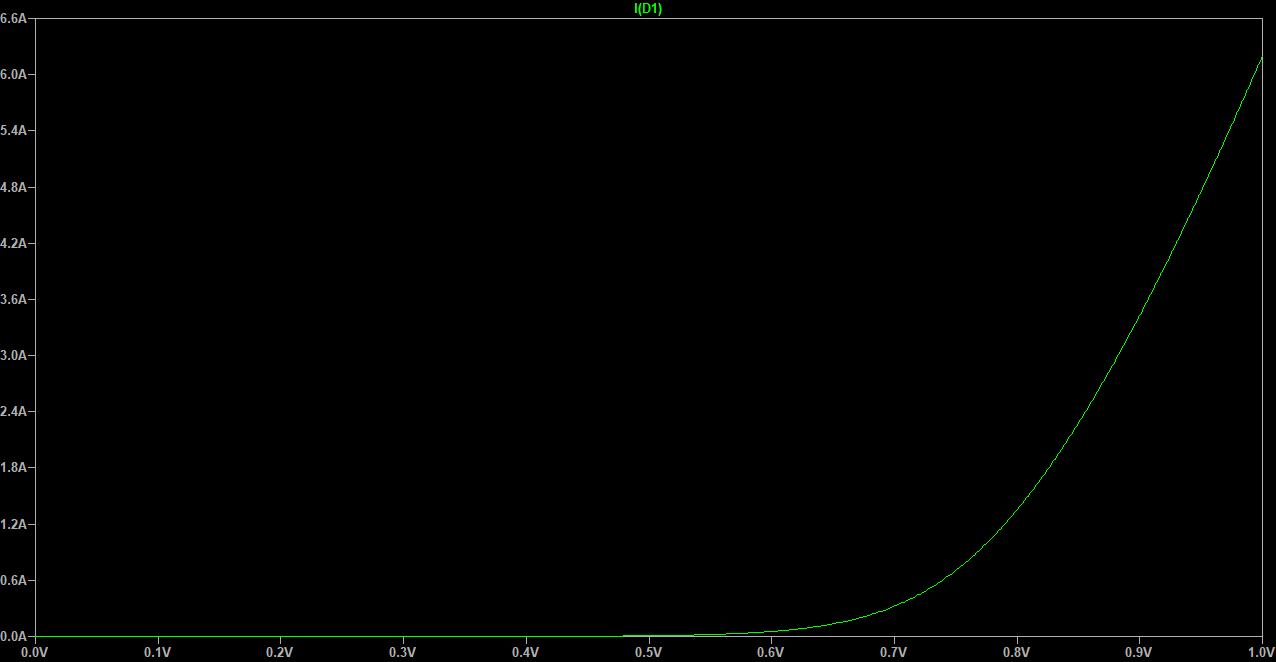
\includegraphics[width=\textwidth]{1_1_vac.png}
    \caption{Прямая ветвь ВАХ.}
    \label{fig:1_1_vac.png}
\end{figure}\\

График похож на экспоненту, что логично, так как аналитически функция \emph{p-n} перехода определяется как:
\[
I = I_0(\exp{\frac{U}{\varphi_T}} - 1),
\]
где $U - $ приложенное к переходу внешнее напряжение соответствующего знака, $I_0 = I_m - $ обратный ток, $\varphi_T = \frac{kT}{q} - $ температурный потенциал. \\
\ \\

Выберем две точки на графике функции для расчета экспериментального сопротивления диода:

\begin{center}
    \begin{tabular}{ |c|c|c|c| } 
    \hline
    № & $I_d$ & $U_d$ & $R_d$\\ 
    \hline
    $1$ & $5.55$ & $0.978$ & $0.176$\\
    \hline
    $2$ & $1.55$ & $0.812$ & $0.524$\\
    \hline
    \end{tabular}
\end{center} \\
Вычислим дифференциальное сопротивление сопротивление смоделированного диода:
\begin{center}
    $R_{diff} = \Delta U / \Delta I = 0.166 / 4 = 0.0415$ Ом
\end{center}
Паспортное значение сопротивления $R_{true} = 0.025$ Ом. Разница между эксперитальным и паспортным значением обуславлиется погрешностью и неоднозначностью выбора точек для расчета.\\
\ \\
Напряжение изгиба $U_{bend} = 0.78$ В.\\
\ \\
Построим полную ВАХ диода:
\begin{figure}[H]
    \centering
    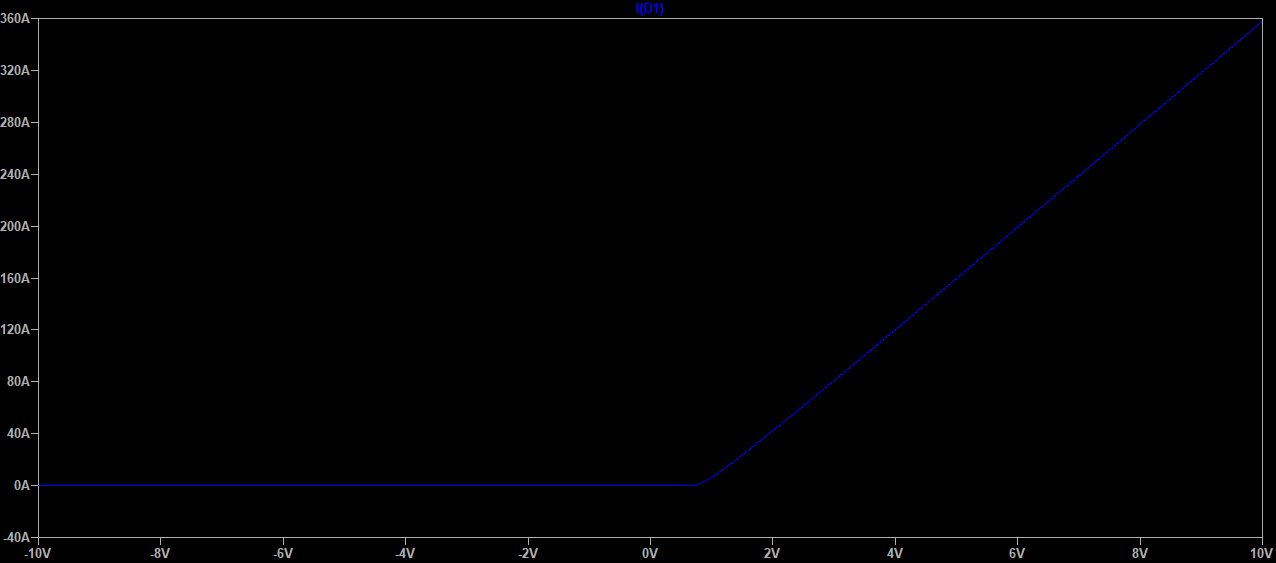
\includegraphics[width=\textwidth]{1_2_vac.png}
    \caption{Полная ветвь ВАХ.}
    \label{fig:1_2_vac.png}
\end{figure}\\
При обратном напряжении сила тока мала (по техническим характеристикам максимальный обратный ток при $T = 25 ^\circ C$ равен $5$ мкА при максимально возможном обратном напряжении $U = 200$ В).\\

\subsubsection*{Исследование работы однополупериодного полупроводникового выпрямителя}
\begin{figure}[H]
    \centering
    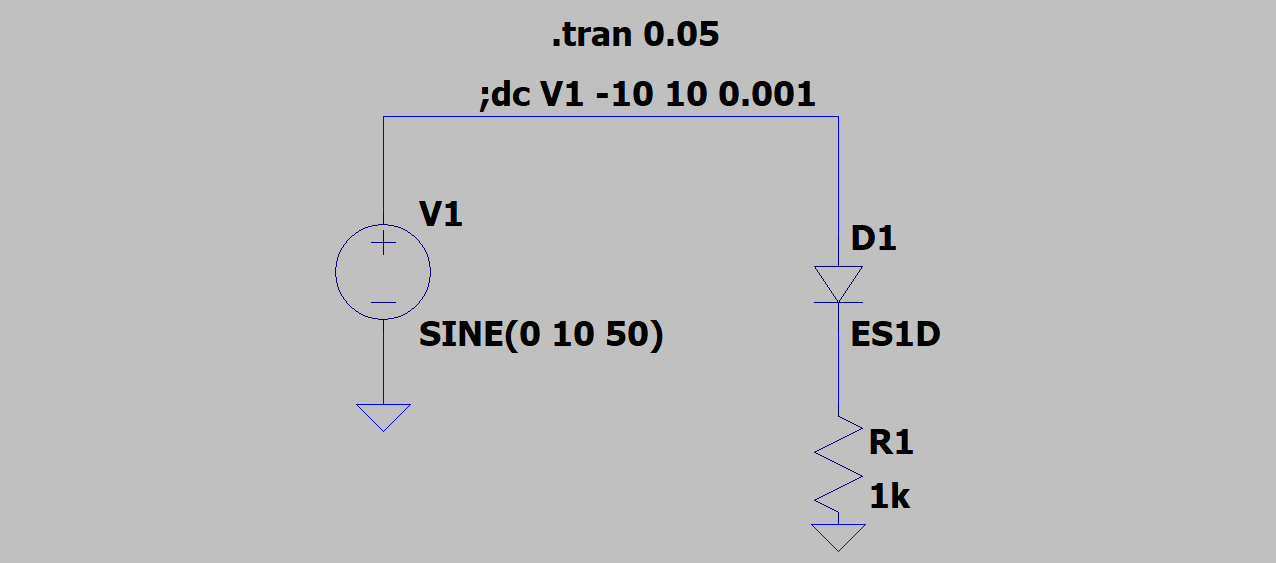
\includegraphics[width=0.7\textwidth]{2_1_circuits_scheme.png}
    \caption{Принципиальная схема для моделирования однофазного однополупериодного выпрямителя.}
    \label{fig:2_1_circuits_scheme.png}
\end{figure}\\

\begin{figure}[H]
    \centering
    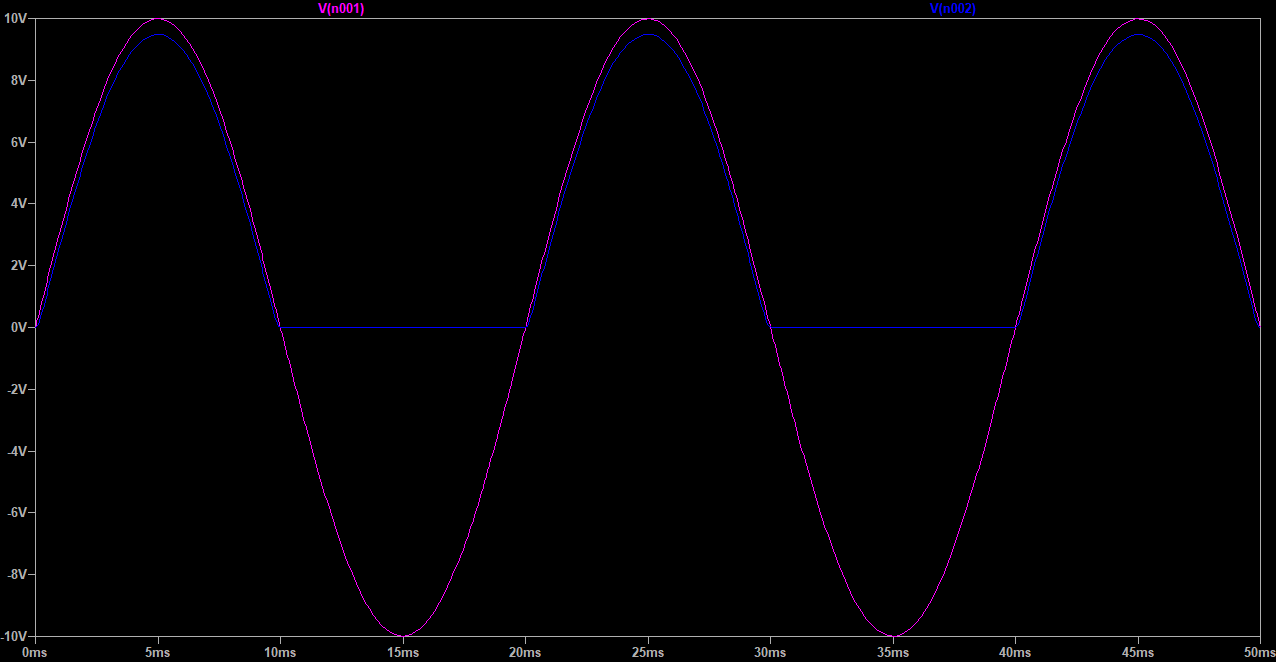
\includegraphics[width=\textwidth]{2_voltages.png}
    \caption{Графики входного и выходного напряжений.}
    \label{fig:2_voltages.png}
\end{figure}\\
Как видно по графику на четных полупериодах напряжение на нагрузке нулевое из-за того, что диод не пропускает ток в обратном направлении. А при нечетных полупериодах направление и ток на нагрузочном резисторе повторяют форму входного сигнала.\\
Также, можем наблюдать потери энергии при прохождении через диод, а именно пик напряжения на нагрузочном резисторе меньше пика входного напряжения.\\
\ \\
Максимальное мгновенное значение напряжения на выходе выпрямителя, определенное по осциллограмме $U_{out_{max}} = 9.46$ В.\\
Средневыпрямленное значение напряжения на выходе диода:
\begin{center}
    $U_{out_{mean}} = U_{out_{max}} / \pi = 3.011$ В.
\end{center}
Максимальное обратное напряжение на диоде $-500$ мкВ.\\
\ \\
Коэффициент пульсации однофазного однополупериодного выпрямителя $k = \frac{\pi}{2}$.\\
Сигнал на выходе выпрямителя имеет тот же период, что и входной сигнал, однако напряжение отсутсвует на половине фазы, следовательно данный выпрямитель неэффективен.

\subsubsection*{Исследование работы однофазного мостового выпрямителя}
\begin{figure}[H]
    \centering
    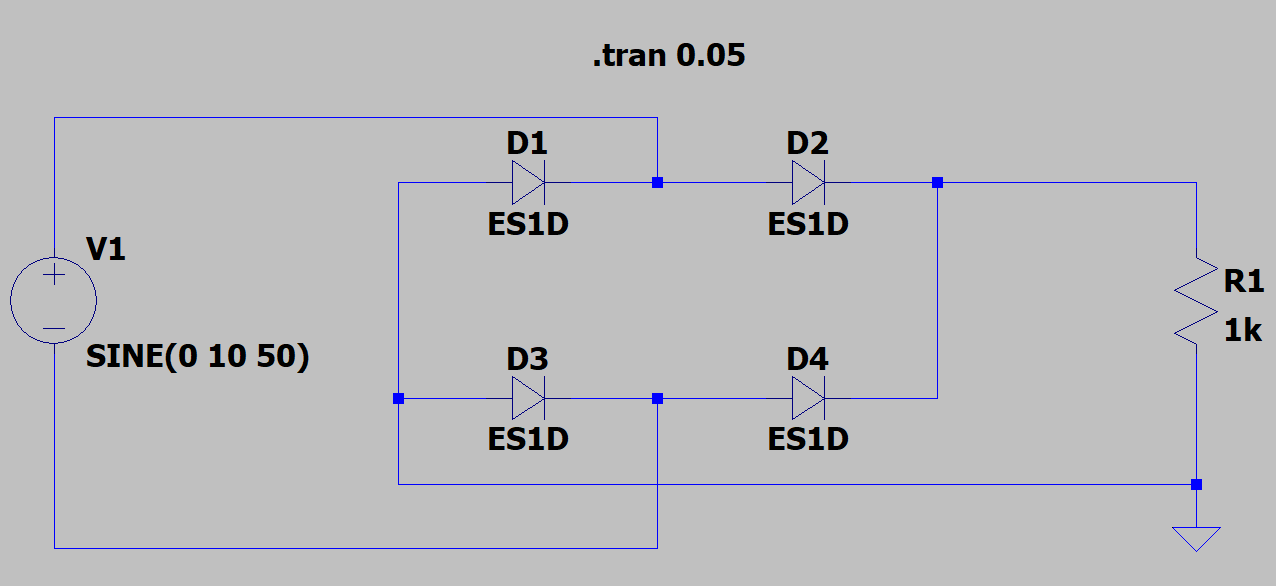
\includegraphics[width=0.7\textwidth]{3_circuits_scheme.png}
    \caption{Принципиальная схема для моделирования однофазного мостового выпрямителя.}
    \label{fig:3_circuits_scheme.png}
\end{figure}\\

\begin{figure}[H]
    \centering
    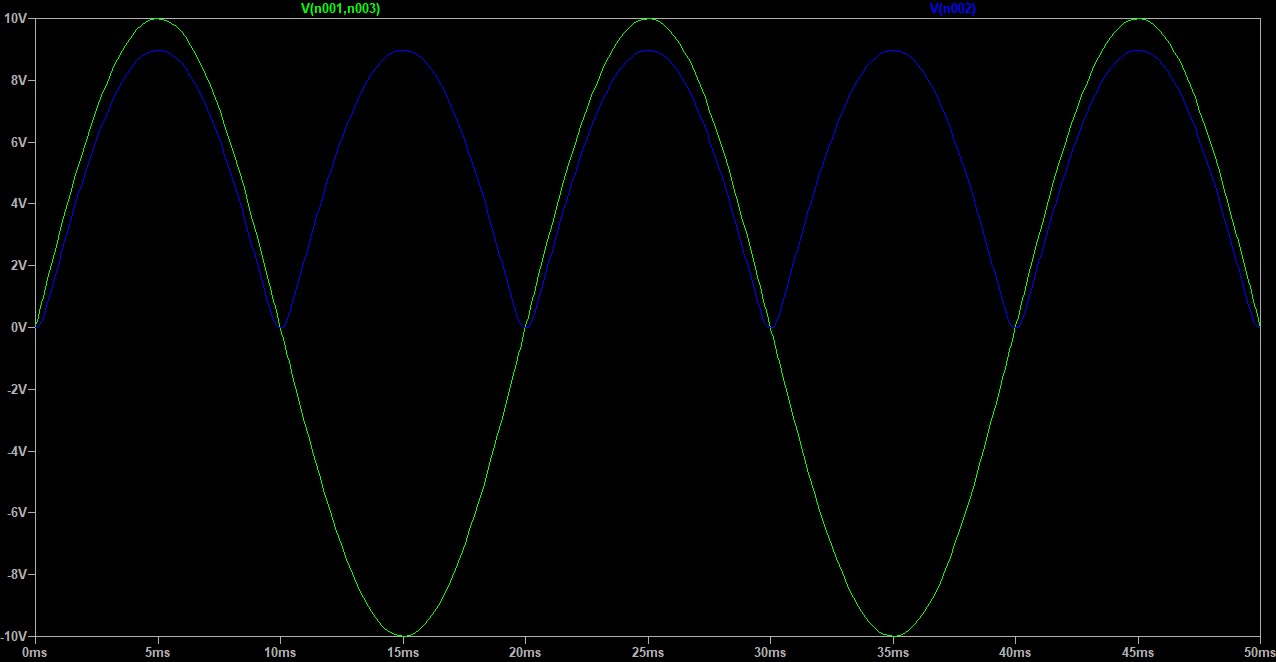
\includegraphics[width=\textwidth]{3_voltages.png}
    \caption{Графики входного и выходного напряжений.}
    \label{fig:3_voltages.png}
\end{figure}\\
Максимальное мгновенное значение напряжения на выходе выпрямителя, определенное по осциллограмме $U_{out_{max}} = 8.973$ В.\\
Заметим, что данное значение меньше аналогичного значения для однополупериодного выпрямителя из прошлого пункта, причиной вероятно служат бОльшие потери энергии из-за прохождения через бОльшее число диодов в цепи.\\
\ \\
Средневыпрямленное значение напряжения на выходе выпрямителя:
\begin{center}
    $U_{out_{mean}} = 2U_{out_{max}} / \pi = 5.712$ В.
\end{center}
\ \\
Коэффициент пульсации однофазного однополупериодного выпрямителя $k = \frac{2}{3}$.\\
Мостовой выпрямитель эффективнее более чем в 2 раза, чем однополупериодный выпрямитель (исходя из значений коэффициента пульсации).\\
Период сигнала на выходе в 2 раза меньше, чем на входе.\\
Однако цель выпрямителя в целом - перевод переменного тока в постоянный, а на осциллограмме мы наблюдаем достаточно сильную пульсацию при смене фаз - это сильный недостаток мостового выпрямителя.

\subsubsection*{Исследование работы однофазного мостового выпрямителя с емкостным сглаживающим фильтром}
Сглаживающий фильтр способен уменьшить пульсации при смене фаз. Он должен пропускать постоянную составляющую выпрямленного напряжения и ослаблять его гармонические составляющие. Для этого используется параллельно подключенный относительно сопротивлению нагрузки конденсатор $C_f$.\\
\ \\
Величину емкости конденсатора необходимо выбрать таким образом, чтобы выполнялось следующее соотношение (при заданном сопротивлении нагрузки):
\[
\omega \cdot R_{load} \cdot C_f = 2 \pi \cdot f \cdot R_{load} \cdot C_f > 1
\]
В нашем случае:
\[
2 \pi \cdot 50 \cdot 1000 \cdot C_f > 1 \Rightarrow C_f > \frac{1}{100 000\pi} \ \text{Ф} \Rightarrow C_f > 3.183\cdot10^{-6} \ \text{Ф}
\]
Итак, выберем значение $C_f = 10$ мкФ.

\begin{figure}[H]
    \centering
    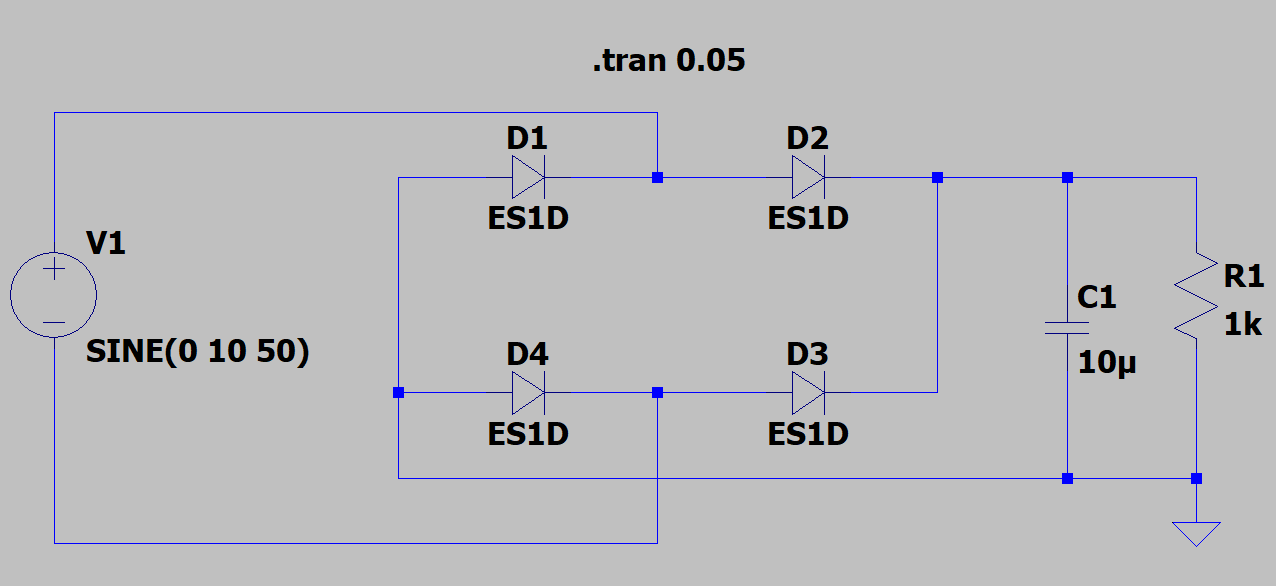
\includegraphics[width=0.7\textwidth]{4_circuits_scheme.png}
    \caption{Принципиальная схема для моделирования однофазного мостового выпрямителя с емкостным сглаживающим фильтром.}
    \label{fig:4_circuits_scheme.png}
\end{figure}\\

\begin{figure}[H]
    \centering
    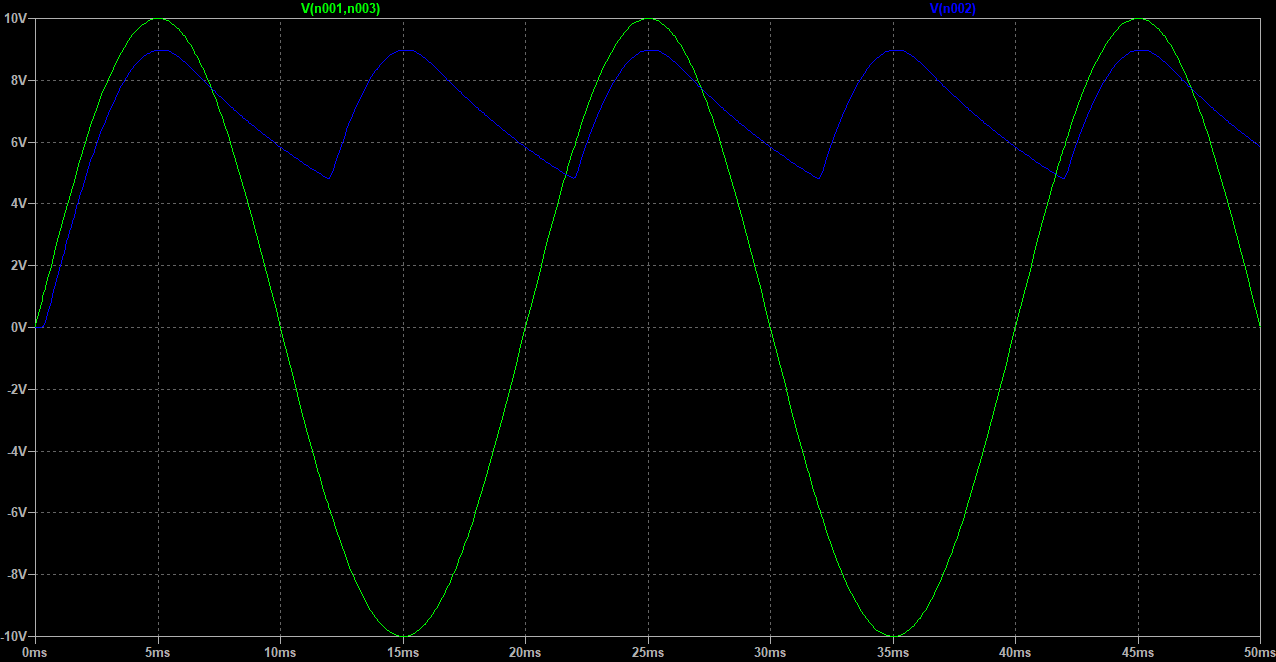
\includegraphics[width=\textwidth]{4_1_voltages.png}
    \caption{Осциллограммы напряжений на входе и выходе выпрямителя.}
    \label{fig:4_1_voltages.png}
\end{figure}\\
Как видим, за счет присутствия конденсатора в схеме выпрямителя пульсации действительно сгладились (это происходит из-за периодического поддержания напряжения на нагрузке зарядом, накопившемся на конденсаторе до этого момента).\\
\ \\
Максимальное и минимальное мгновенные значения напряжения на выходе выпрямителя, определенные по осциллограмме:
\[
U_{out_{max}} = 8.980 \ \text{В} , \ U_{out_{min}} = 4.818 \ \text{В}.
\]
Максимальное значение совпадает с максимальным в случае обычного мостового выпрямителя, а вот минимальное значение, которые (мы и стремились приблизить к верхней границе) увеличилось.\\
\ \\
Среднее значение выходного сигнала: $U_{{out}_{mean}} = 6.9282$ В.\\
Коэффициент пульсации:
\[
k = \frac{U_{out_{max}} - U_{out_{min}}}{U_{{out}_{mean}}} = 0.6007
\]
Работа выпрямителя с емкостным фильтром эффективнее, так как мы видим по осциллограммам более устойчивый, менее пульсирующий выходной ток по сравнению с обычным мостовым выпрямителем.\\
Это подтверждает и меньшее значение коэффициента пульсации (выпрямитель с фильтром эффективнее на $ 10\% $).\\

\paragraph*{Увеличенная частота входного сигнала}
\ \\
Увеличим частоту входного сигнала до максимально допустимой $200$ Гц.
\begin{figure}[H]
    \centering
    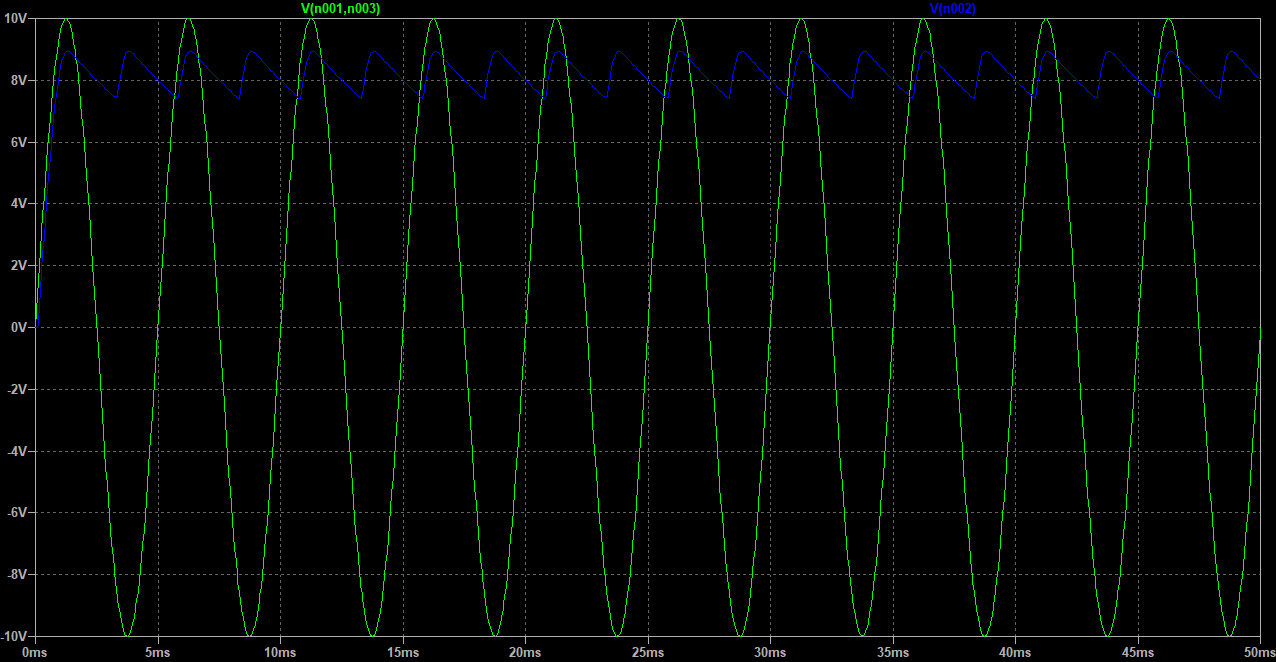
\includegraphics[width=\textwidth]{4_inc_voltage.png}
    \caption{Осциллограммы напряжений на входе и выходе выпрямителя при $200$ Гц.}
    \label{fig:4_inc_voltage.png}
\end{figure}\\
Максимальное и минимальное мгновенные значения напряжения на выходе выпрямителя, определенные по осциллограмме:
\[
U_{out_{max}} = 8.942 \ \text{В} , \ U_{out_{min}} = 7.407 \ \text{В}.
\]
Среднее значение выходного сигнала: $U_{{out}_{mean}} = 8.1473$ В.\\
Коэффициент пульсации:
\[
k = \frac{U_{out_{max}} - U_{out_{min}}}{U_{{out}_{mean}}} = 0.1884
\]
Увеличение частоты входного сигнала положительно влияет на характер выходного тока - коэффициент пульсации снижается.\\
\ \\
Так как мы знаем, что формула зависимости нарастания напряжения от времени заряда в конденсаторе имеет вид: 
\[
U = U_{out}(1 - \exp{-t/T}),
\]
где $U_{out}$ – электродвижущая сила источника, $t$ - время заряда, $T$ - постоянная времени, равная $R\cdot C$.\\
Следовательно, до определенной частоты конденсатор будет успевать накапливать такой же заряд (как в случае идентичной системы, но с меньшей частотой), а значит из-за бОльшей частоты смены фазы (в этот момент напряжение поддерживается за счёт зарядов, накопленных в конденсаторе) напряжение не успевает упасть так, как в системе с меньшей частотой.\\

\paragraph*{Увеличенная емкость конденсатора}
\ \\
Увеличим емкость конденсатора в 10 раз до $100$ мкФ.
\begin{figure}[H]
    \centering
    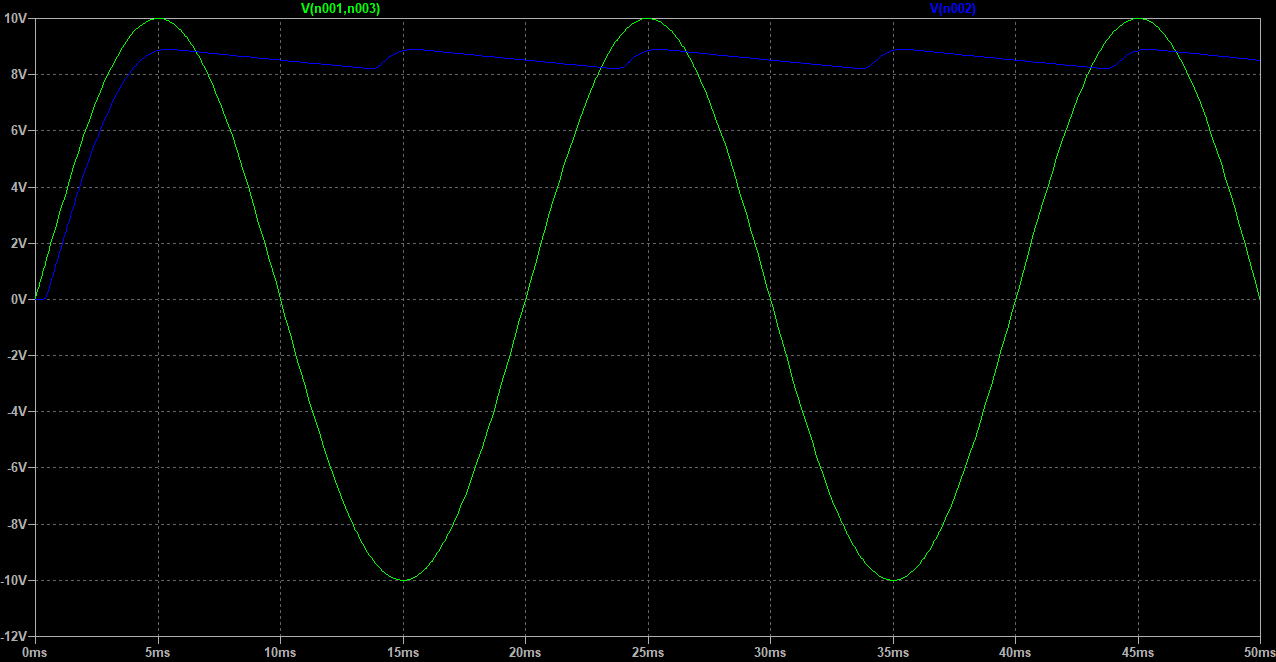
\includegraphics[width=\textwidth]{4_inc_capacity.png}
    \caption{Осциллограммы напряжений на входе и выходе выпрямителя при $C_f = 100$ мкФ.}
    \label{fig:4_inc_capacity.png}
\end{figure}\\
Максимальное и минимальное мгновенные значения напряжения на выходе выпрямителя, определенные по осциллограмме:
\[
U_{out_{max}} = 8.898 \ \text{В} , \ U_{out_{min}} = 8.212 \ \text{В}.
\]
Среднее значение выходного сигнала: $U_{{out}_{mean}} = 8.2354$ В.\\
Коэффициент пульсации:
\[
k = \frac{U_{out_{max}} - U_{out_{min}}}{U_{{out}_{mean}}} = 0.0833
\]
Очевидно, что при увеличении емкости конденсатора, он способен накапливать бОльший заряд и, следовательно, при смене фазы падение напряжения будет значительно меньше, так как оно будет поддерживаться на уровне из зарядов, накопленных на конденсаторе (конденсатор не успевает полностью разряжаться).\\
Следовательно мы видим достаточно хороший выпрямленный ток, практически без пульсаций.

\paragraph*{Прямоугольный сигнал}

\begin{figure}[H]
    \centering
    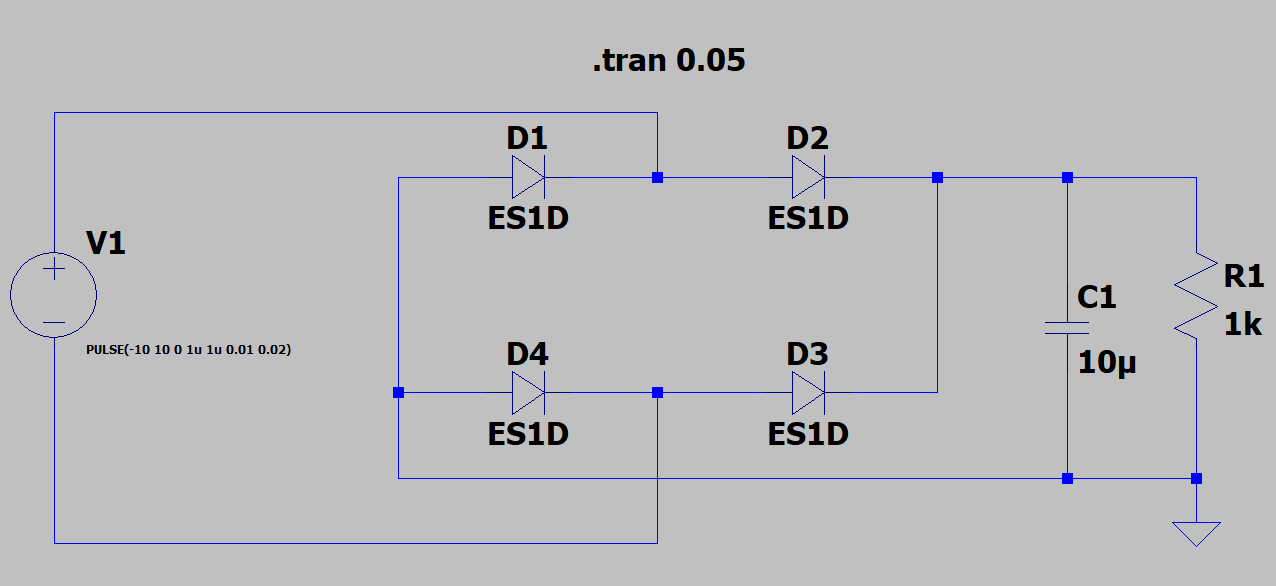
\includegraphics[width=0.7\textwidth]{4_rect_signal.png}
    \caption{Принципиальная схема для моделирования выпрямителя с прямоугольным сигналом.}
    \label{fig:4_rect_signal.png}
\end{figure}\\

\begin{figure}[H]
    \centering
    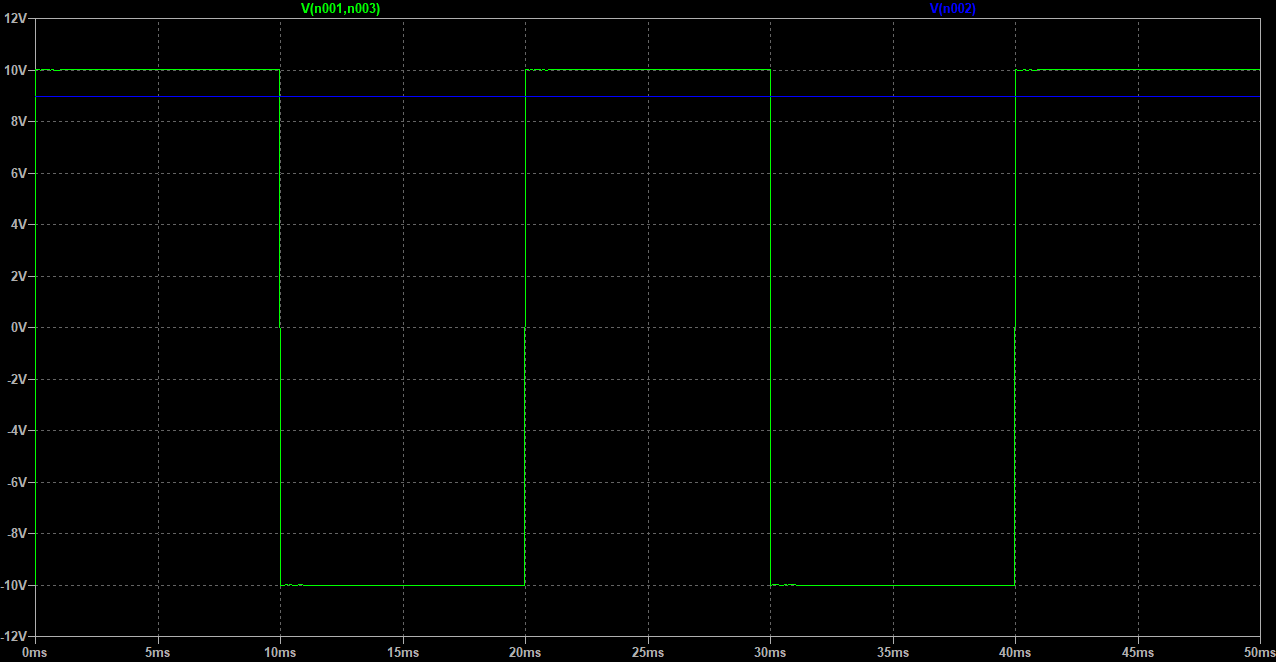
\includegraphics[width=\textwidth]{4_rect_voltages.png}
    \caption{Осциллограммы напряжений на входе и выходе выпрямителя при прямоугольном сигнале.}
    \label{fig:4_rect_voltages.png}
\end{figure}\\

Максимальное, минимальное мгновенные и среднее значения напряжения на выходе выпрямителя равны:
\[
U_{out_{max}} = U_{out_{min}} = U_{{out}_{mean}} = 8.986 \ \text{В}.
\]
Коэффициент пульсации:
\[
k = \frac{U_{out_{max}} - U_{out_{min}}}{U_{{out}_{mean}}} = 0
\]
При данном сигнале мы получаем идеально выпрямленный ток (коэффициент пульсации $0$). Это происходит, так как конденсатор успевает накопить достаточно заряда для того, чтобы скомпенсировать недостающее напряжение при смене фаз.

\paragraph*{Треугольный сигнал}

\begin{figure}[H]
    \centering
    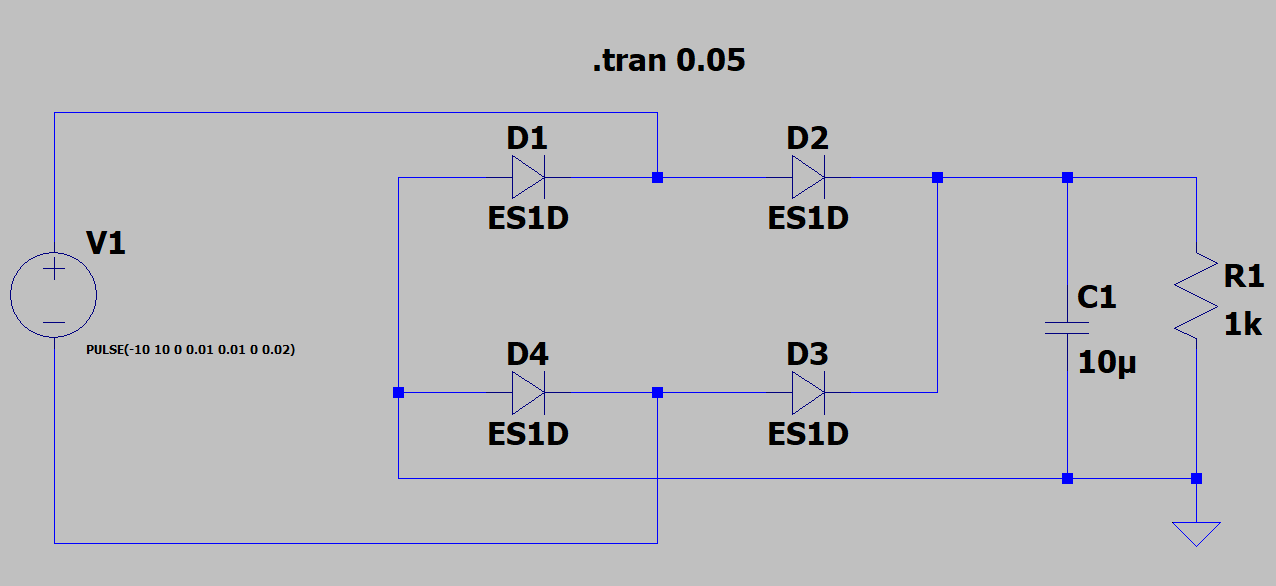
\includegraphics[width=0.7\textwidth]{4_triangular_signal.png}
    \caption{Принципиальная схема для моделирования выпрямителя с треугольным сигналом.}
    \label{fig:4_triangular_signal.png}
\end{figure}\\

\begin{figure}[H]
    \centering
    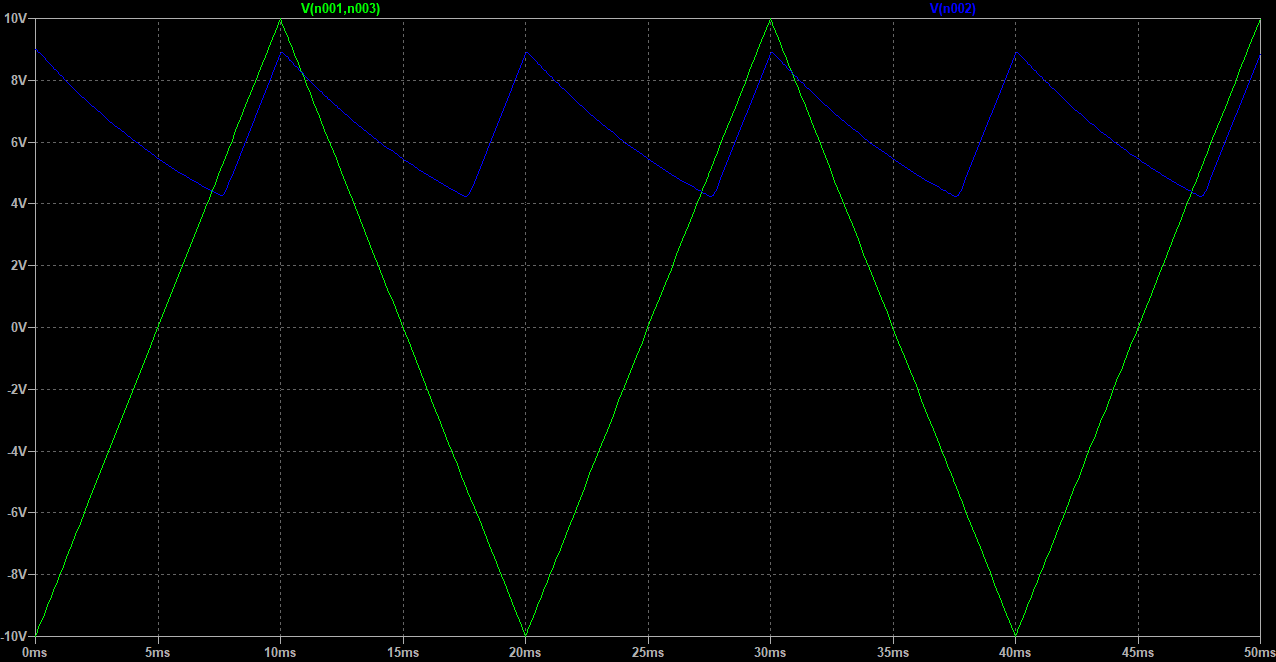
\includegraphics[width=\textwidth]{4_triangular_voltages.png}
    \caption{Осциллограммы напряжений на входе и выходе выпрямителя при треугольном сигнале.}
    \label{fig:4_triangular_voltages.png}
\end{figure}\\

Максимальное и минимальное мгновенные значения напряжения на выходе выпрямителя, определенные по осциллограмме:
\[
U_{out_{max}} = 8.895 \ \text{В}, \ U_{out_{min}} = 4.236 \ \text{В}.
\]
Среднее значение выходного сигнала:
\[
U_{{out}_{mean}} = 6.3495 \ \text{В}.
\]
Коэффициент пульсации:
\[
k = \frac{U_{out_{max}} - U_{out_{min}}}{U_{{out}_{mean}}} = 0.7336
\]
Результаты данного эксперимента в целом схожи с аналогичным периодическим синусоидальным входным воздействием, однако там выпрямитель справлялся лучше (при всех аналогичным параметрах сети, $k_{sin} = 0.6007$). Так как синусоидальный сигнал имеет бОльшее среднее значение сигнала и, следовательно, конденсатор заряжается на бОльший заряд.

\paragraph*{Пилообразный сигнал}

\begin{figure}[H]
    \centering
    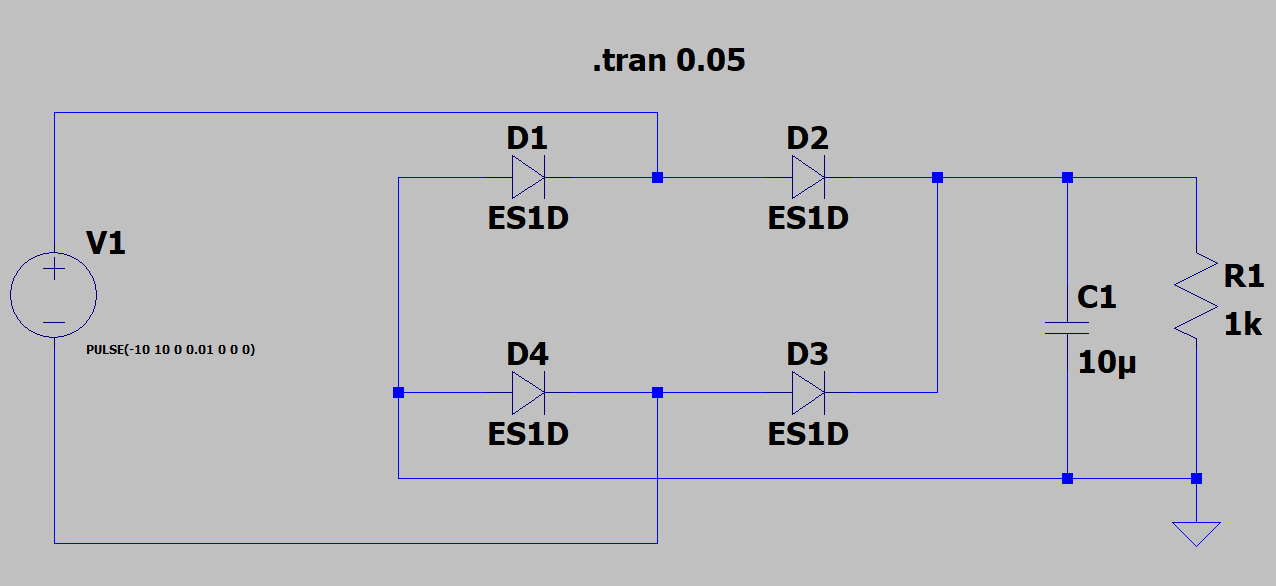
\includegraphics[width=0.7\textwidth]{4_saw_signal.png}
    \caption{Принципиальная схема для моделирования выпрямителя с пилообразным сигналом.}
    \label{fig:4_saw_signal.png}
\end{figure}\\

\begin{figure}[H]
    \centering
    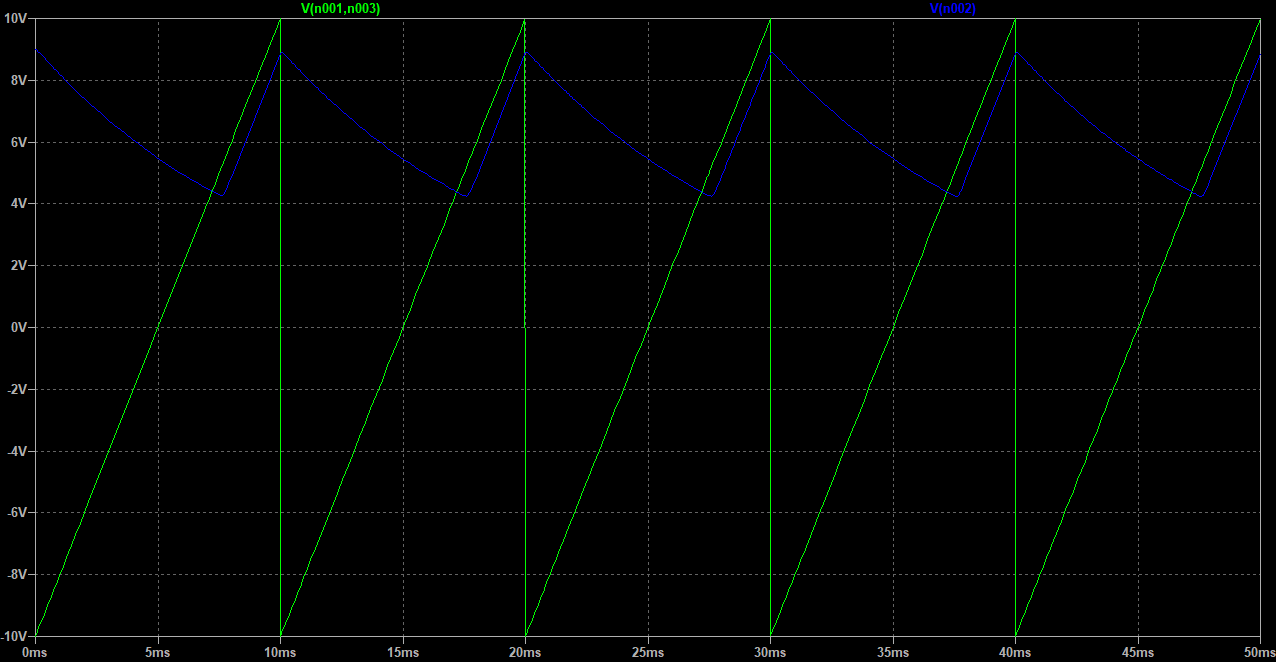
\includegraphics[width=\textwidth]{4_saw_voltages.png}
    \caption{Осциллограммы напряжений на входе и выходе выпрямителя при пилообразным сигнале.}
    \label{fig:4_saw_voltages.png}
\end{figure}\\

Максимальное и минимальное мгновенные значения напряжения на выходе выпрямителя, определенные по осциллограмме:
\[
U_{out_{max}} = 8.896 \ \text{В}, \ U_{out_{min}} = 4.241 \ \text{В}.
\]
Среднее значение выходного сигнала:
\[
U_{{out}_{mean}} = 6.3496 \ \text{В}.
\]
Коэффициент пульсации:
\[
k = \frac{U_{out_{max}} - U_{out_{min}}}{U_{{out}_{mean}}} = 0.7278
\]
Результаты эксперимента при пилообразном сигнале практически идентичны эксперименту с трегольным сигналом.

\section*{Выводы}
В данной лабораторной работе были исследованы принципы работы выпрямительных диодов при различных параметрах.\\
Наиболее эффектривным из рассмотренных выпрямителем является мостовой выпрямитель с емкостным сглаживающим фильтром. Оценка эффективности проводилась по значению коэффициента пульсаций $k$ (чем меньше, тем эффективнее выпрямление тока).
Работу данного выпрямителя можно улучшить увеличением емкости конденсатора.\\
При различных типах и частотах входного сигнала эффективность работы мостовогот выпрямителя с емкостным фильтром разная (при увеличении частоты входного сигнала до определенного значения эффектвность возрастает). 

\end{document}